\documentclass[convert={density=300,outext=.png}]{standalone}
\usepackage{tikz}

\begin{document}
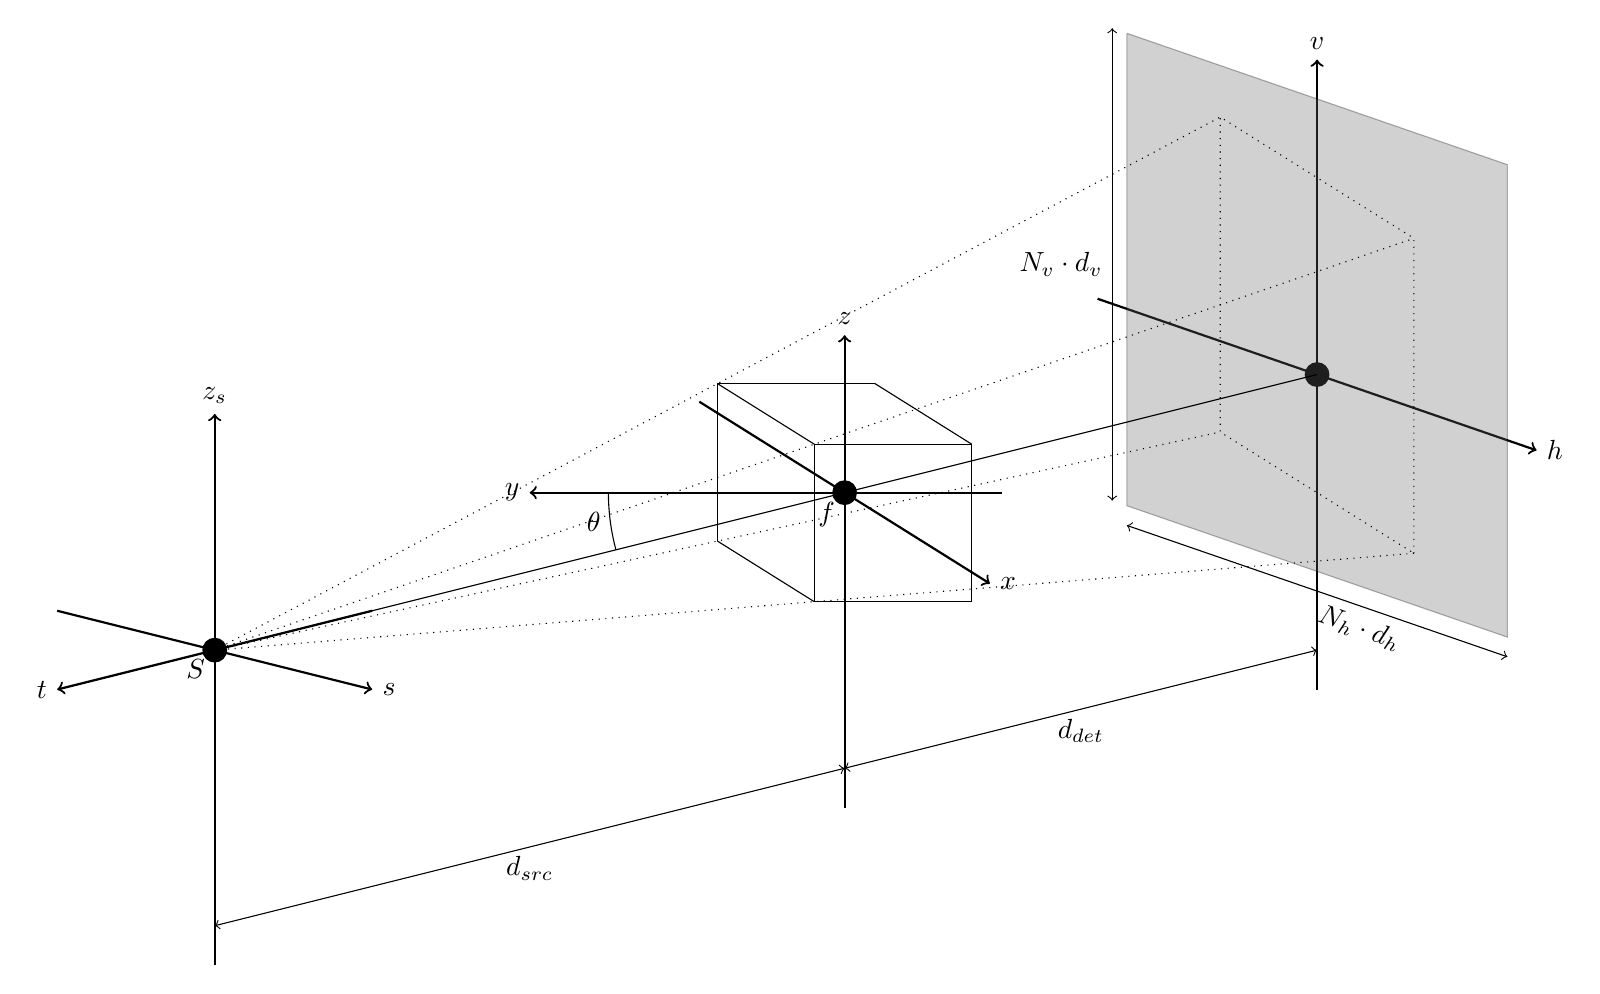
\begin{tikzpicture}[axis/.style={thick,->}]
    % Quelle
    \coordinate (1) at (0, 0, 0);
    \filldraw[fill=black,draw=black] (1) circle (0.15cm) node[below left] {$S$};
    \draw[axis] (-2, 0.5, 0) -- (2, -0.5, 0) node[right] {$s$};
    \draw[axis] (2, 0.5, 0) -- (-2, -0.5, 0) node[left] {$t$};
    \draw[axis] (0, -4, 0) -- (0, 3, 0) node[above] {$z_s$};

    % Volumen
    \coordinate (2) at (8, 2, 0);
    \filldraw[fill=black,draw=black] (2) circle (0.15cm) node[below left] {$f$};
    \draw[axis] (5, 2, -3) -- (11, 2, 3) node[right] {$x$};
    \draw[axis] (10, 2, 0) -- (4, 2, 0) node[left] {$y$};
    \draw[axis] (8, -2, 0) -- (8, 4, 0) node[above] {$z$};

    \draw (8, 1, 1) -- (10, 1, 1);
    \draw (8, 1, 1) -- (8, 3, 1);
    \draw (8, 1, 1) -- (6, 1, -1);

    \draw (8, 3, 1) -- (10, 3, 1);
    \draw (8, 3, 1) -- (6, 3, -1);

    \draw (10, 1, 1) -- (10, 3, 1);

    \draw (6, 1, -1) -- (6, 3, -1);

    \draw (6, 3, -1) -- (8, 3, -1);

    \draw (10, 3, 1) -- (8, 3, -1);


    % Detektor
    \coordinate(3) at (14, 3.5, 0);
    \filldraw[fill=black,draw=black] (3) circle (0.15cm);
    \draw[axis] (10.25, 3.5, -2.5) -- (17.75, 3.5, 2.5) node[right] {$h$};
    \draw[axis] (14, -0.5, 0) -- (14, 7.5, 0) node[above] {$v$};
    \draw[fill=black!60!white,opacity=0.3] (10.75, 7, -2.16666) -- (17.25, 7, 2.16666) -- (17.25, 1, 2.16666)
                                           -- (10.75, 1, -2.16666) -- (10.75, 7, -2.16666);
    \draw[<->] (10.5, 1, -2.33333) -- (10.5, 7, -2.33333) node[pos=0.5, left] {$N_v \cdot d_v$};
    \draw[<->] (10.75, 0.75, -2.16666) -- (17.25, 0.75, 2.16666) node[pos=0.5,sloped,below right] {$N_h \cdot d_h$};

    % Abstände
    \draw (1) -- (3);
    \draw[<->] (0, -3.5, 0) -- (8, -1.5, 0) node[pos=0.5,below] {$d_{src}$};
    \draw[<->] (8, -1.5, 0) -- (14, 0, 0) node[pos=0.5,below] {$d_{det}$};

    % Kegelstrahlen
    \draw[dotted] (1) -- (16, 2, 2);
    \draw[dotted] (1) -- (16, 6, 2);
    \draw[dotted] (1) -- (12, 2, -2);
    \draw[dotted] (1) -- (12, 6, -2);

    % Kegelstrahlenabbild
    \draw[dotted] (16, 2, 2) -- (16, 6, 2) -- (12, 6, -2) -- (12, 2, -2) -- (16, 2, 2);

    % Winkel
    \draw (5, 2, 0) arc (180:195:2.8cm) node[pos=0.5, left] {$\theta$};
\end{tikzpicture}
\end{document}
